\documentclass{article}

% formatting
\usepackage[utf8]{inputenc} % allow utf-8 input
\usepackage[T1]{fontenc} % use 8-bit T1 fonts  (allows for direct use of ö,ü,etc.)

% math typesetting
\usepackage{amsmath}
\usepackage{amsfonts}

% color
\usepackage{color}
\usepackage{xcolor}

% layout
\usepackage{layout}
\usepackage{lipsum}

% cross-referencing and hyperlinks
\usepackage{hyperref}
\usepackage{url}
\usepackage{doi}

% figures
\usepackage{graphicx}

% tables
\usepackage{booktabs}
\usepackage{multirow}
\usepackage{caption} 
\usepackage{float}

% enumeration
\usepackage{enumitem}

% embedding pages
\usepackage{pdfpages}

% multi-line comments
\usepackage{comment}

% footnotes
\usepackage{footnote}

\usepackage{subfig}
\usepackage{cleveref}

\usepackage[
    backend=biber,
    style=authoryear-comp
]{biblatex}
\addbibresource{references.bib}

%%%%%%%%%%%%%%%%%%%%%%%%%%%%%%%%%%%%%%%%%%%%%%%%%%%%%%%%%%%%%%%%%%%%%

% document metadata
\title{Proposal for a Summer Academy of the Swiss Study Foundation}
\author{Michael Weinold, Philippe Schultheiss et al.}
\date{2023}

%%%%%%%%%%%%%%%%%%%%%%%%%%%%%%%%%%%%%%%%%%%%%%%%%%%%%%%%%%%%%%%%%%%%%

\begin{document}

\maketitle

\section{Authors}

Michael Weinold is a doctoral researcher at ETH Zurich and the Paul Scherrer Institute. With a background in physics, his academic research has been centered around accelerating innovation in clean-energy technologies. For his doctoral research project, he is improving the mathematical modeling of life-cycle assessment methods. A student of history and enthusiastic draftsman, he XXXX. Originally from Innsbruck, Austria.

Philippe Schultheiss is a philosopher who is currently training to become a priest with the reformed church of Zurich. 

Mark Christopher Ballandies is a crypto whale.

\section{Abstract}

We must reduce global carbon emissions dramatically. The construction sector is responsible for XX\% of annual global carbon emissions. In Switzerland, it accounts for XX\% of carbon emissions (including imported carbon). This number is expected to increase to XX\% in 2050, due to strong immigration.
What is more, the construction sector is notoriously difficult to decarbonise. Together with certain heavy industry sectors and aviation, it is classified as a "hard to abate" sector.
Work is ongoing on decreasing the carbon footprint of building during the construction phase and during the use phase. This includes novel methods for cement, concrete and steel production or the increasing digitisation of buildings ("smart home"). However, there are currently no efforts to increase the lifetime of buildings. In Switzerland, like in the surrounding EU countries, average building lifetime is around 50 years only.
The carbon emissions incurred during new construction of a building vs the refurbishment can be recouped over a period of between XX-XX years. Studies exist for the nordic countries, where the energy cost of non-refurbished buildings is highest. Average building lifetimes are between 50 years (France, with source) and 60 years (Switzerland, with source).
Despite efforts to improve recycling in construction, recycling rate of modern building materials (steel, concrete, glass) remains low (check for source).
[Figure from Crawford on cumulative embodied energy]
At the same time, changing use requirements meet the modernist credo "form follows function". Changing family structures mean that apartments can be ever more compact.
All this amounts to large scale new construction, the majority of which is in the 'modernist' or contemporary style.
Every poll to date has shown that this style is at the very least moderately unpopular with people. Empirical evidence is mounting, thereby providing proof for something that has been well-known to the general public for a long time: "Why is the Modern World So Ugly?" (Alain de Boton)




A key reason for the short lifetime of buildings is the 

\tableofcontents

\section{Introduction}

\begin{figure}[]
    \centering
    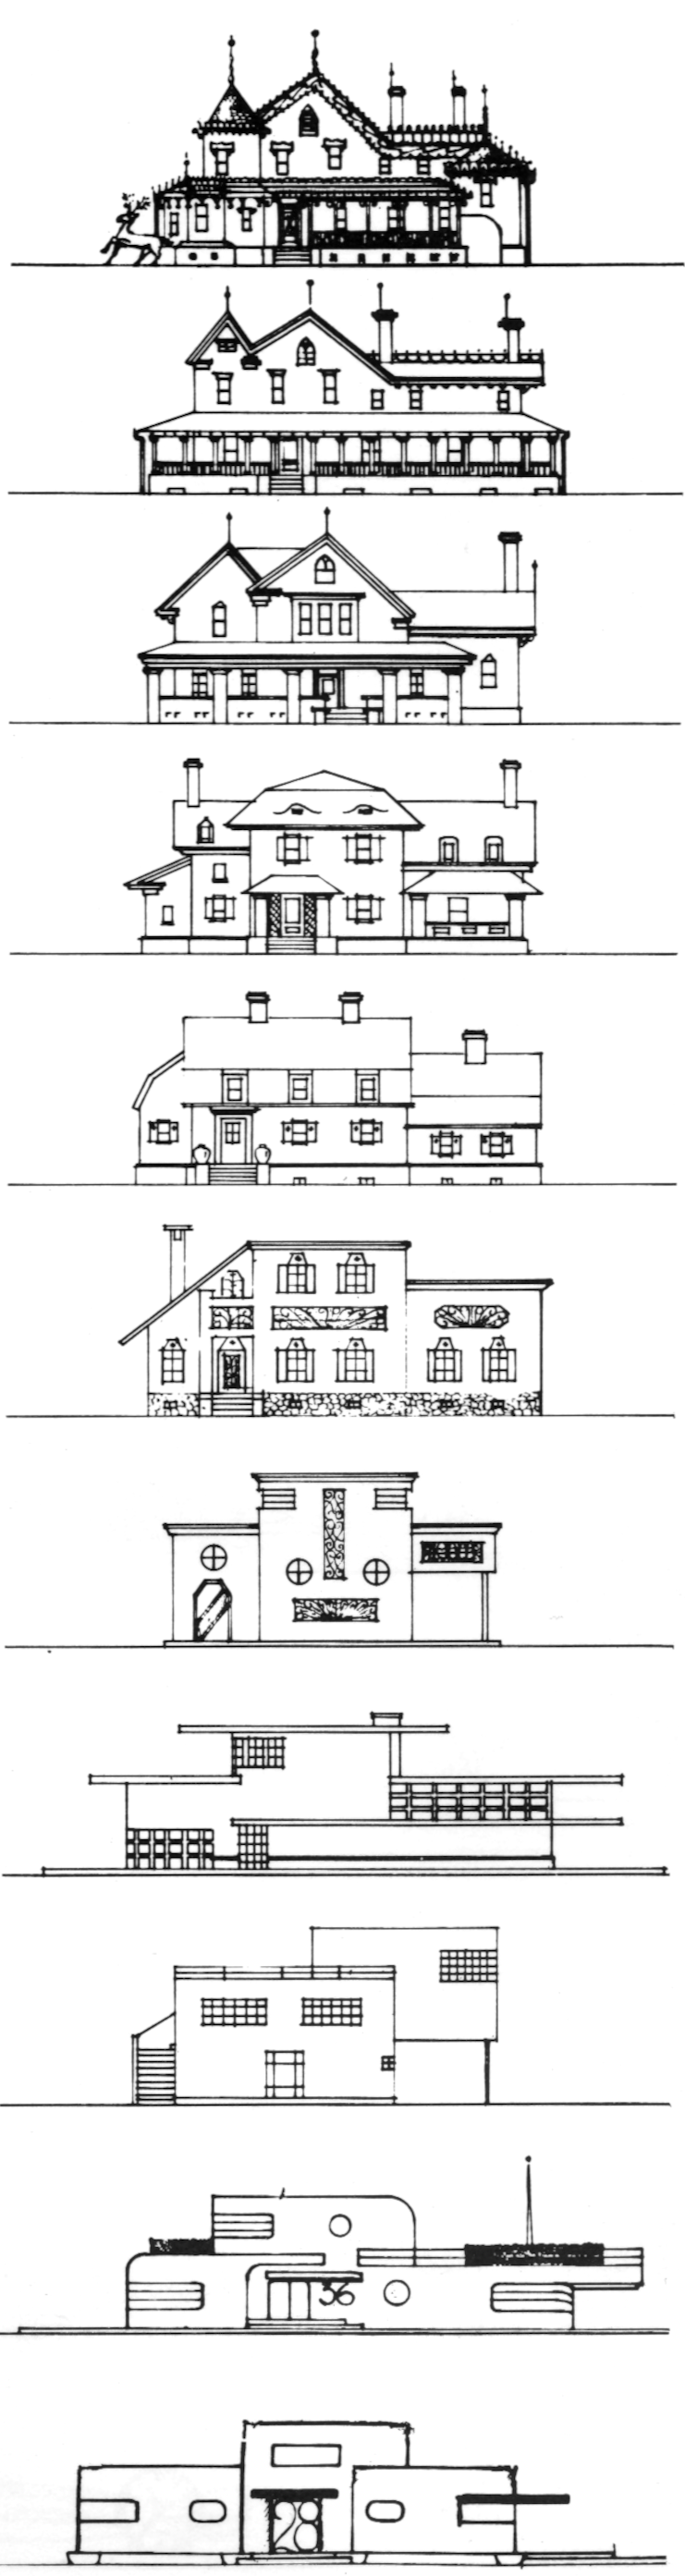
\includegraphics[height=\textheight]{./figures/loewy_architecture.png}
    \caption{
        Some text here. Source: "Design Evolution 1930", \cite{loewy_industrial_1979}
    }
    \label{fig:combined}
\end{figure}

\section{Scope of the Discussion}

Modern architecture is always ugly. Nonetheless, we limit our discussion to buildings of a representative nature. We exclude housing (eg. apartment complexes) to avoid:

\section{Scattered Thoughts}

Architects have been publicly calling for the public to be re-educated to appreciate their brutalist/modernist designs. (eg. the architects that build the Triemli Tower).

Some potential pathways to decarbonizing the economy are difficult for technical and political reasons. This includes "flying less", "reducing personal mobility", etc.
However, some aspects should be really simple: "don't design houses for a 50 year lifetime"

\section{Sustainability}

\section{Aesthetics}

\textit{"[Architecture] (...) is the most overweening of the arts, and the one that least lets us alone. A gallery we can't walk out of, a book we can't close, an art we can't even turn our back on because it is there facing us on the other side of the street as well (...)} - British poet Blake Morrison in "Lords of glass, steel and concrete" \cite{morrison_lords_1982}

\section{Connecting Aesthetics and Sustainability}



Studies show that 

\begin{figure}
    \centering
    \subfloat{{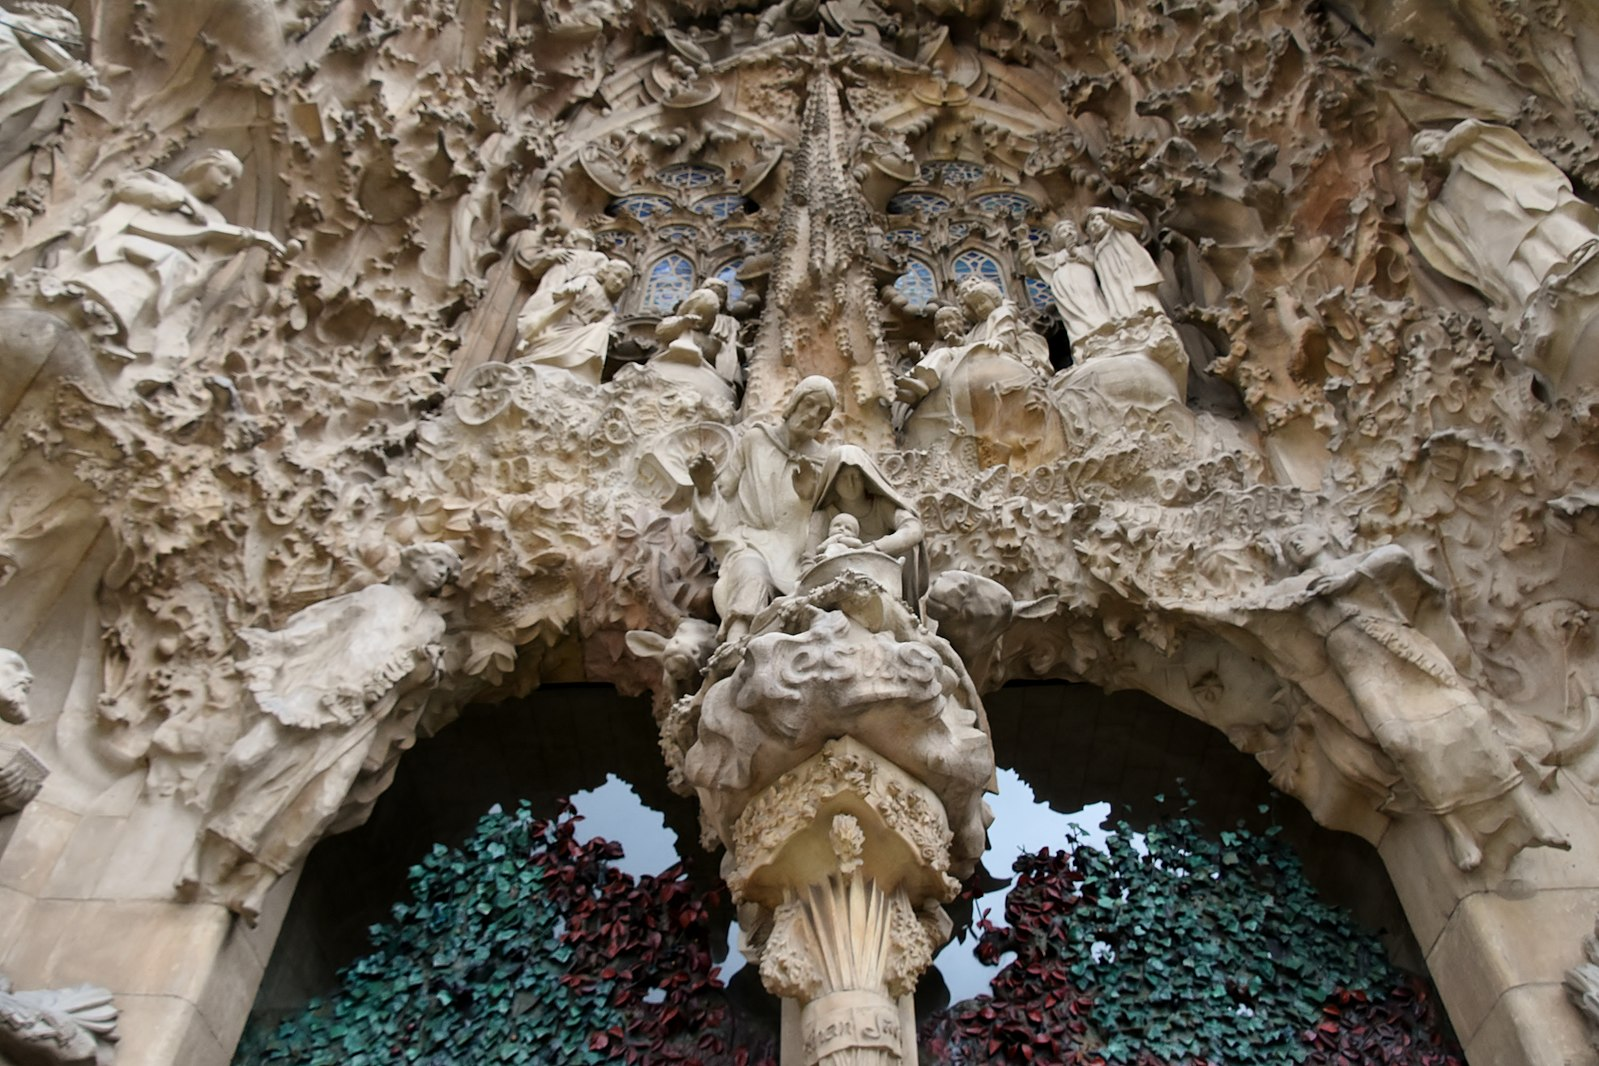
\includegraphics[height=4cm]{figures/sagrada_facade.jpg} }}
    \subfloat{{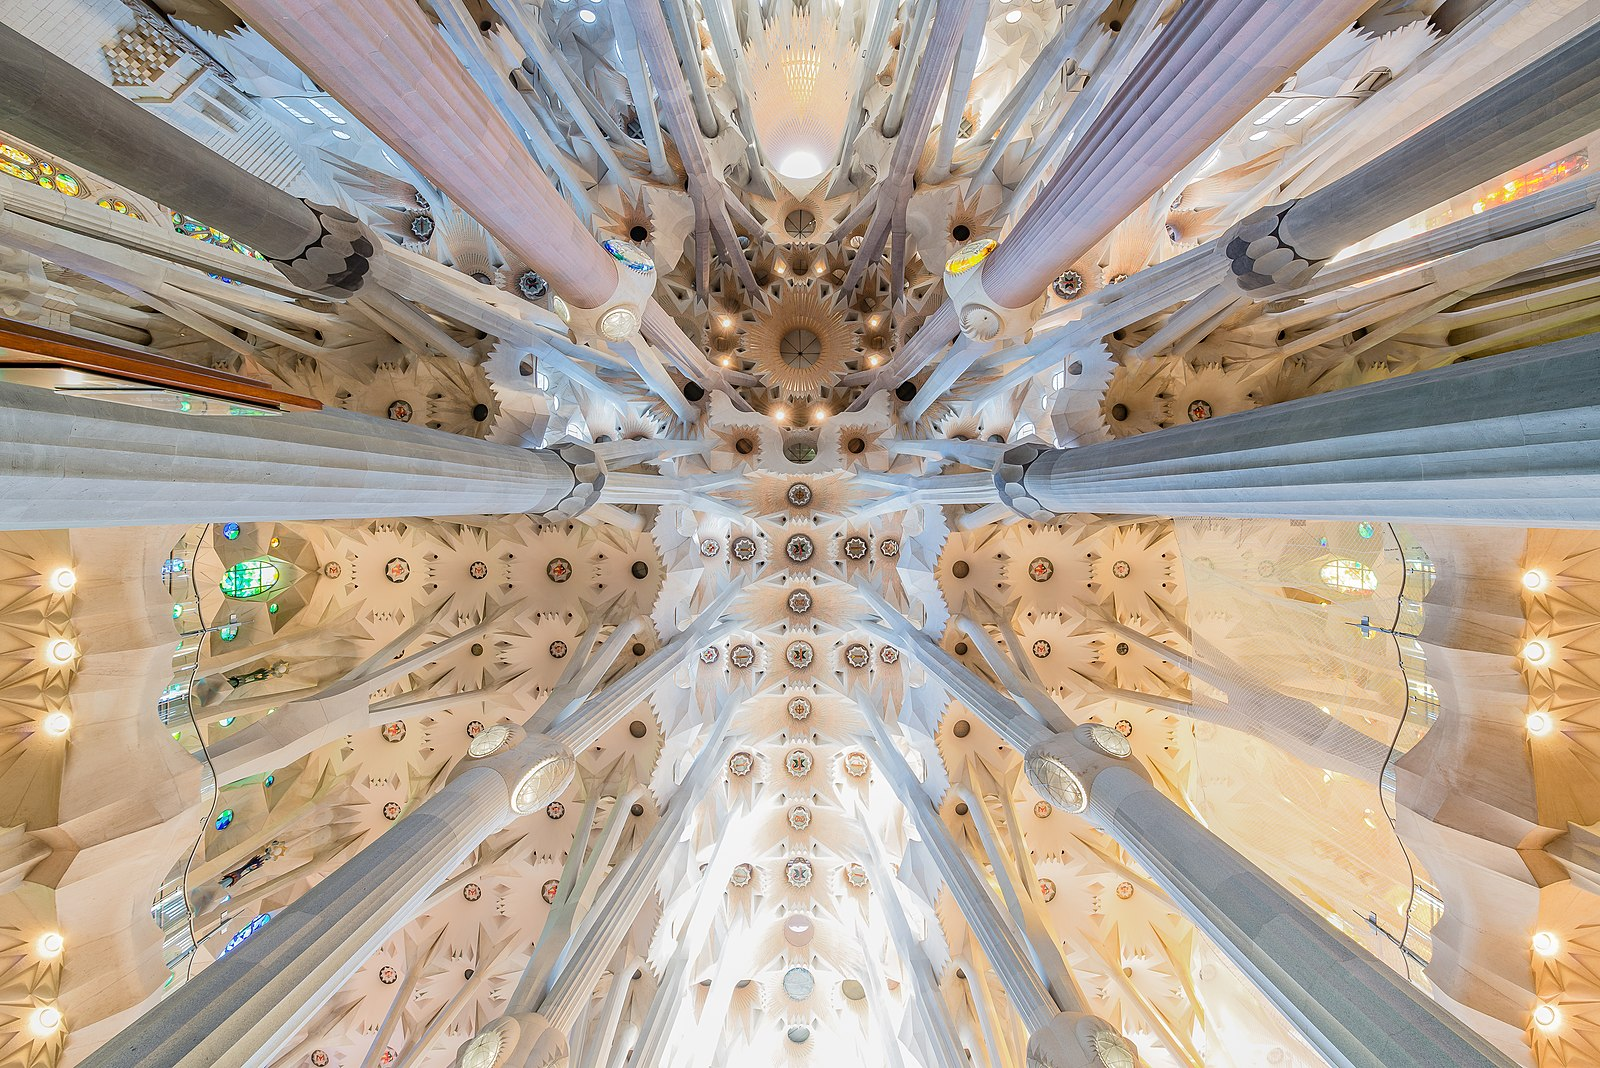
\includegraphics[height=4cm]{figures/sagrada_interior.jpg} }}
    \caption{Gothic Revival, Art Nouveau and Modernista catholic church "Sagrada Familia" (en.: "Holy Family") in Barcelona, Spain, designed by Antoni Gaudí from 1883 until his death in 1926. Left: Detail of the nativity façade with XXXX. Right: Wide-angle view of the   Image sources from left to right: Outside view \cite{mortel_sagrada_2016} and inside view \cite{wikimedia_commons_user_t_meltzer_sagrada_2014}.}
    \label{fig:kunstformen}
\end{figure}

\begin{figure}
    \centering
    \subfloat{{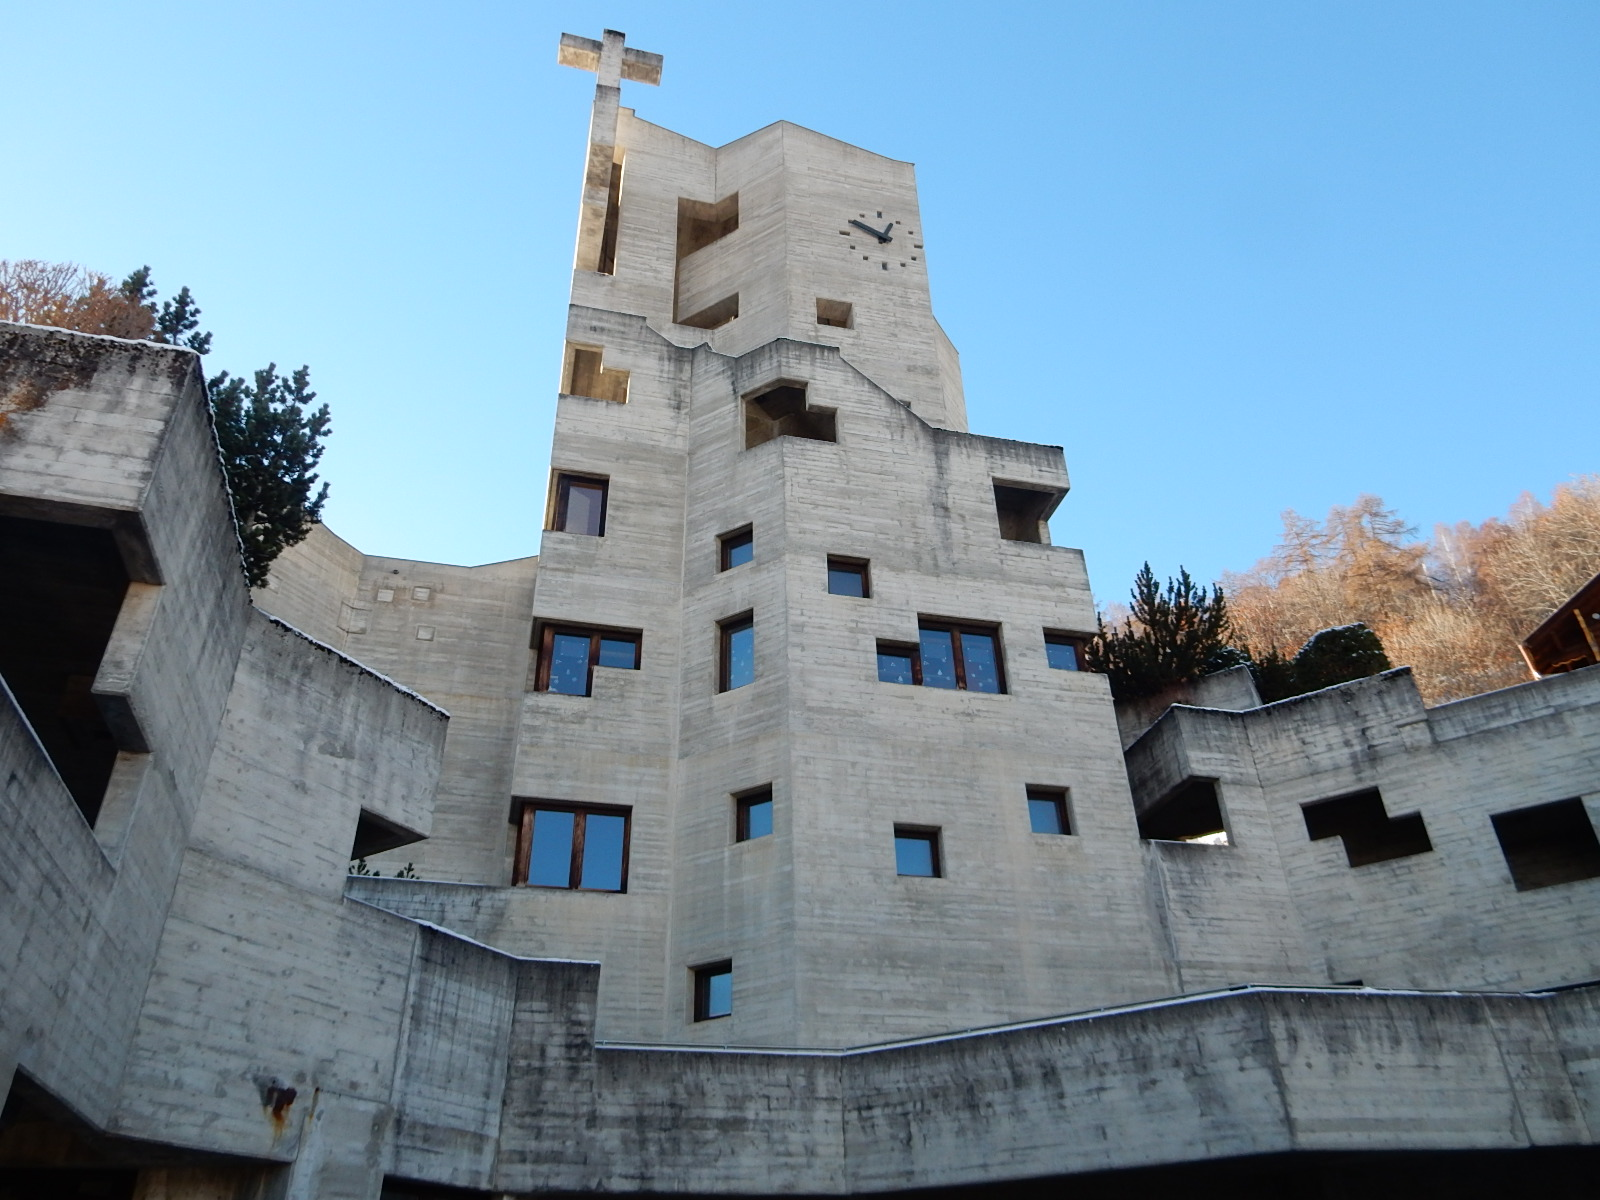
\includegraphics[height=4.5cm]{figures/hérémence_1.jpg} }}
    \subfloat{{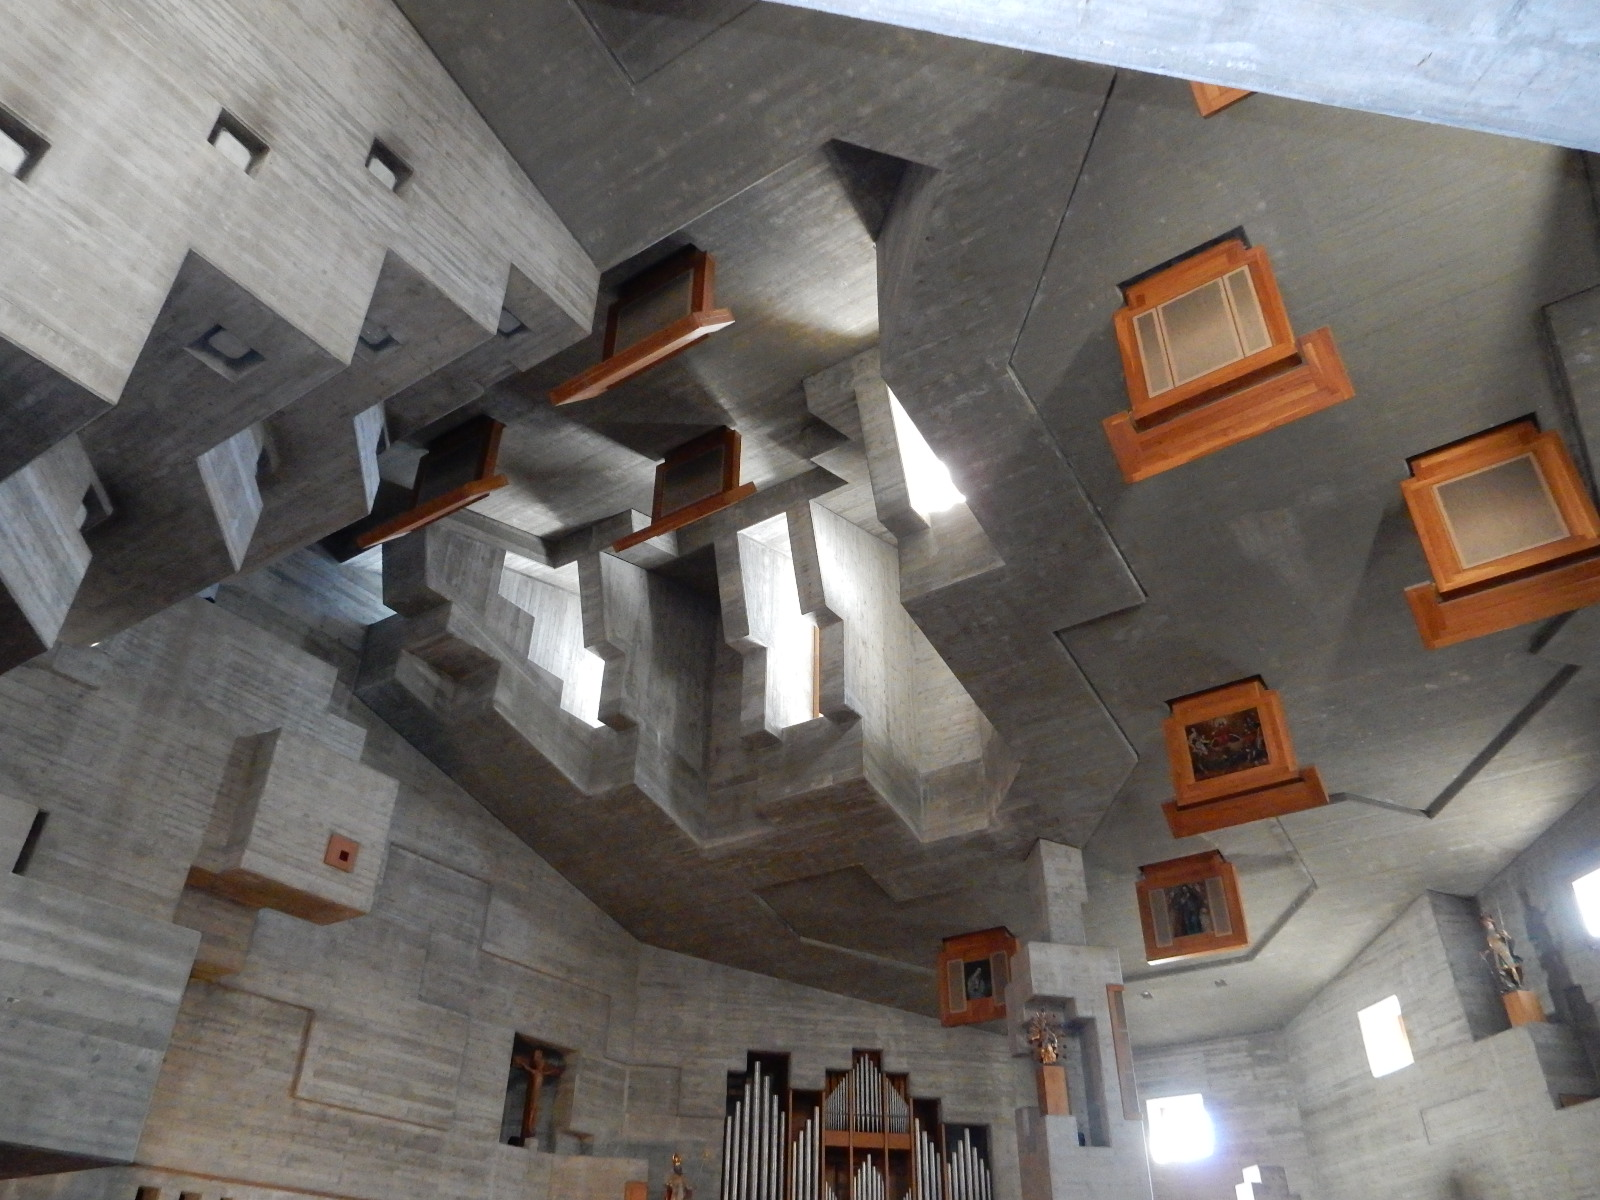
\includegraphics[height=4.5cm]{figures/hérémence_2.jpg} }}
    \caption{Brutalist-style catholic church "St. Nicolas" in the Swiss mountain village of Hérémence, designed by Walter Maria Förderer in 1967. Image sources from left to right: Outside view \cite{bissegger_eglise_2018-1} and inside view \cite{bissegger_eglise_2018}.}
    \label{fig:kunstformen}
\end{figure}

\newpage

\begin{figure}
    \centering
    \subfloat{{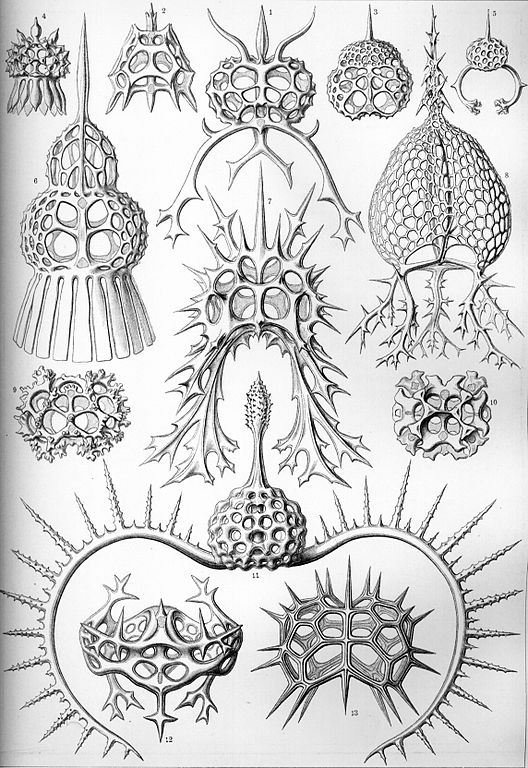
\includegraphics[height=5.5cm]{figures/Spyroidea.jpg} }}
    \subfloat{{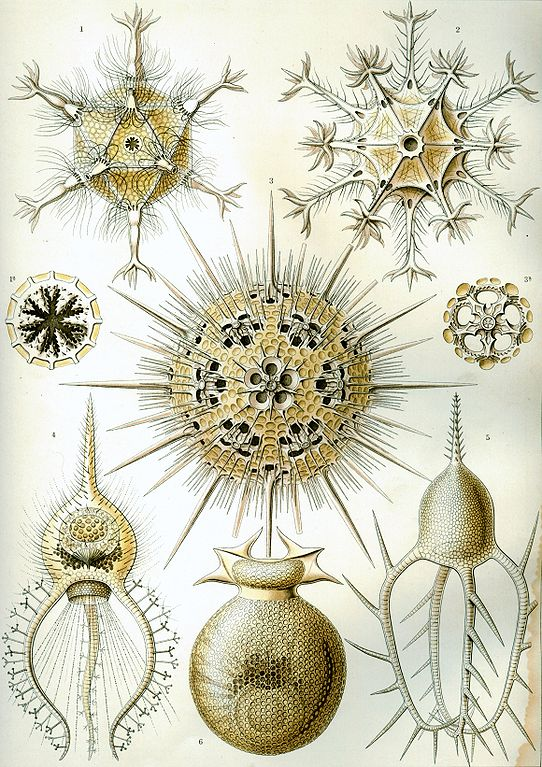
\includegraphics[height=5.5cm]{figures/Phaeodaria.jpg} }}
    \subfloat{{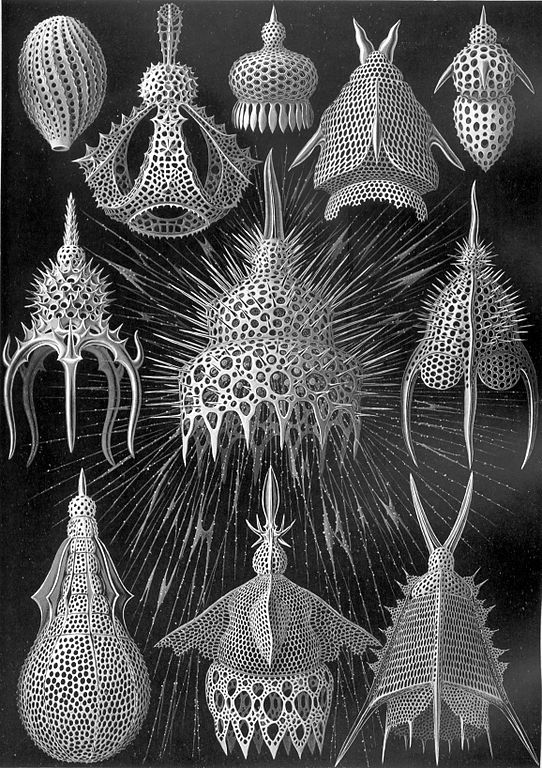
\includegraphics[height=5.5cm]{figures/Cyrtoidea.jpg} }}
    \caption{Selection of drawings from Ernst Haeckel's \textit{"Kunstformen der Natur" (en.: "Art Forms in Nature")} \cite{haeckel_kunstformen_2012}. According to Rene Binet, drawings like these served as inspiration for his monumental arch \cite[Sec. "Haeckel und der Jugendstil"]{willmann_haeckel_2019}, which is depicted in \cref{fig:arch}. Image sources from left to right: Spyroidea \cite{haeckel_kunstformen_1904}, Phaeodaria \cite{haeckel_kunstformen_1904} and Cyrtoidea \cite{haeckel_kunstformen_1904-2} by Ernst Haeckel.}
    \label{fig:kunstformen}
\end{figure}

\begin{figure}
    \centering
    \subfloat{{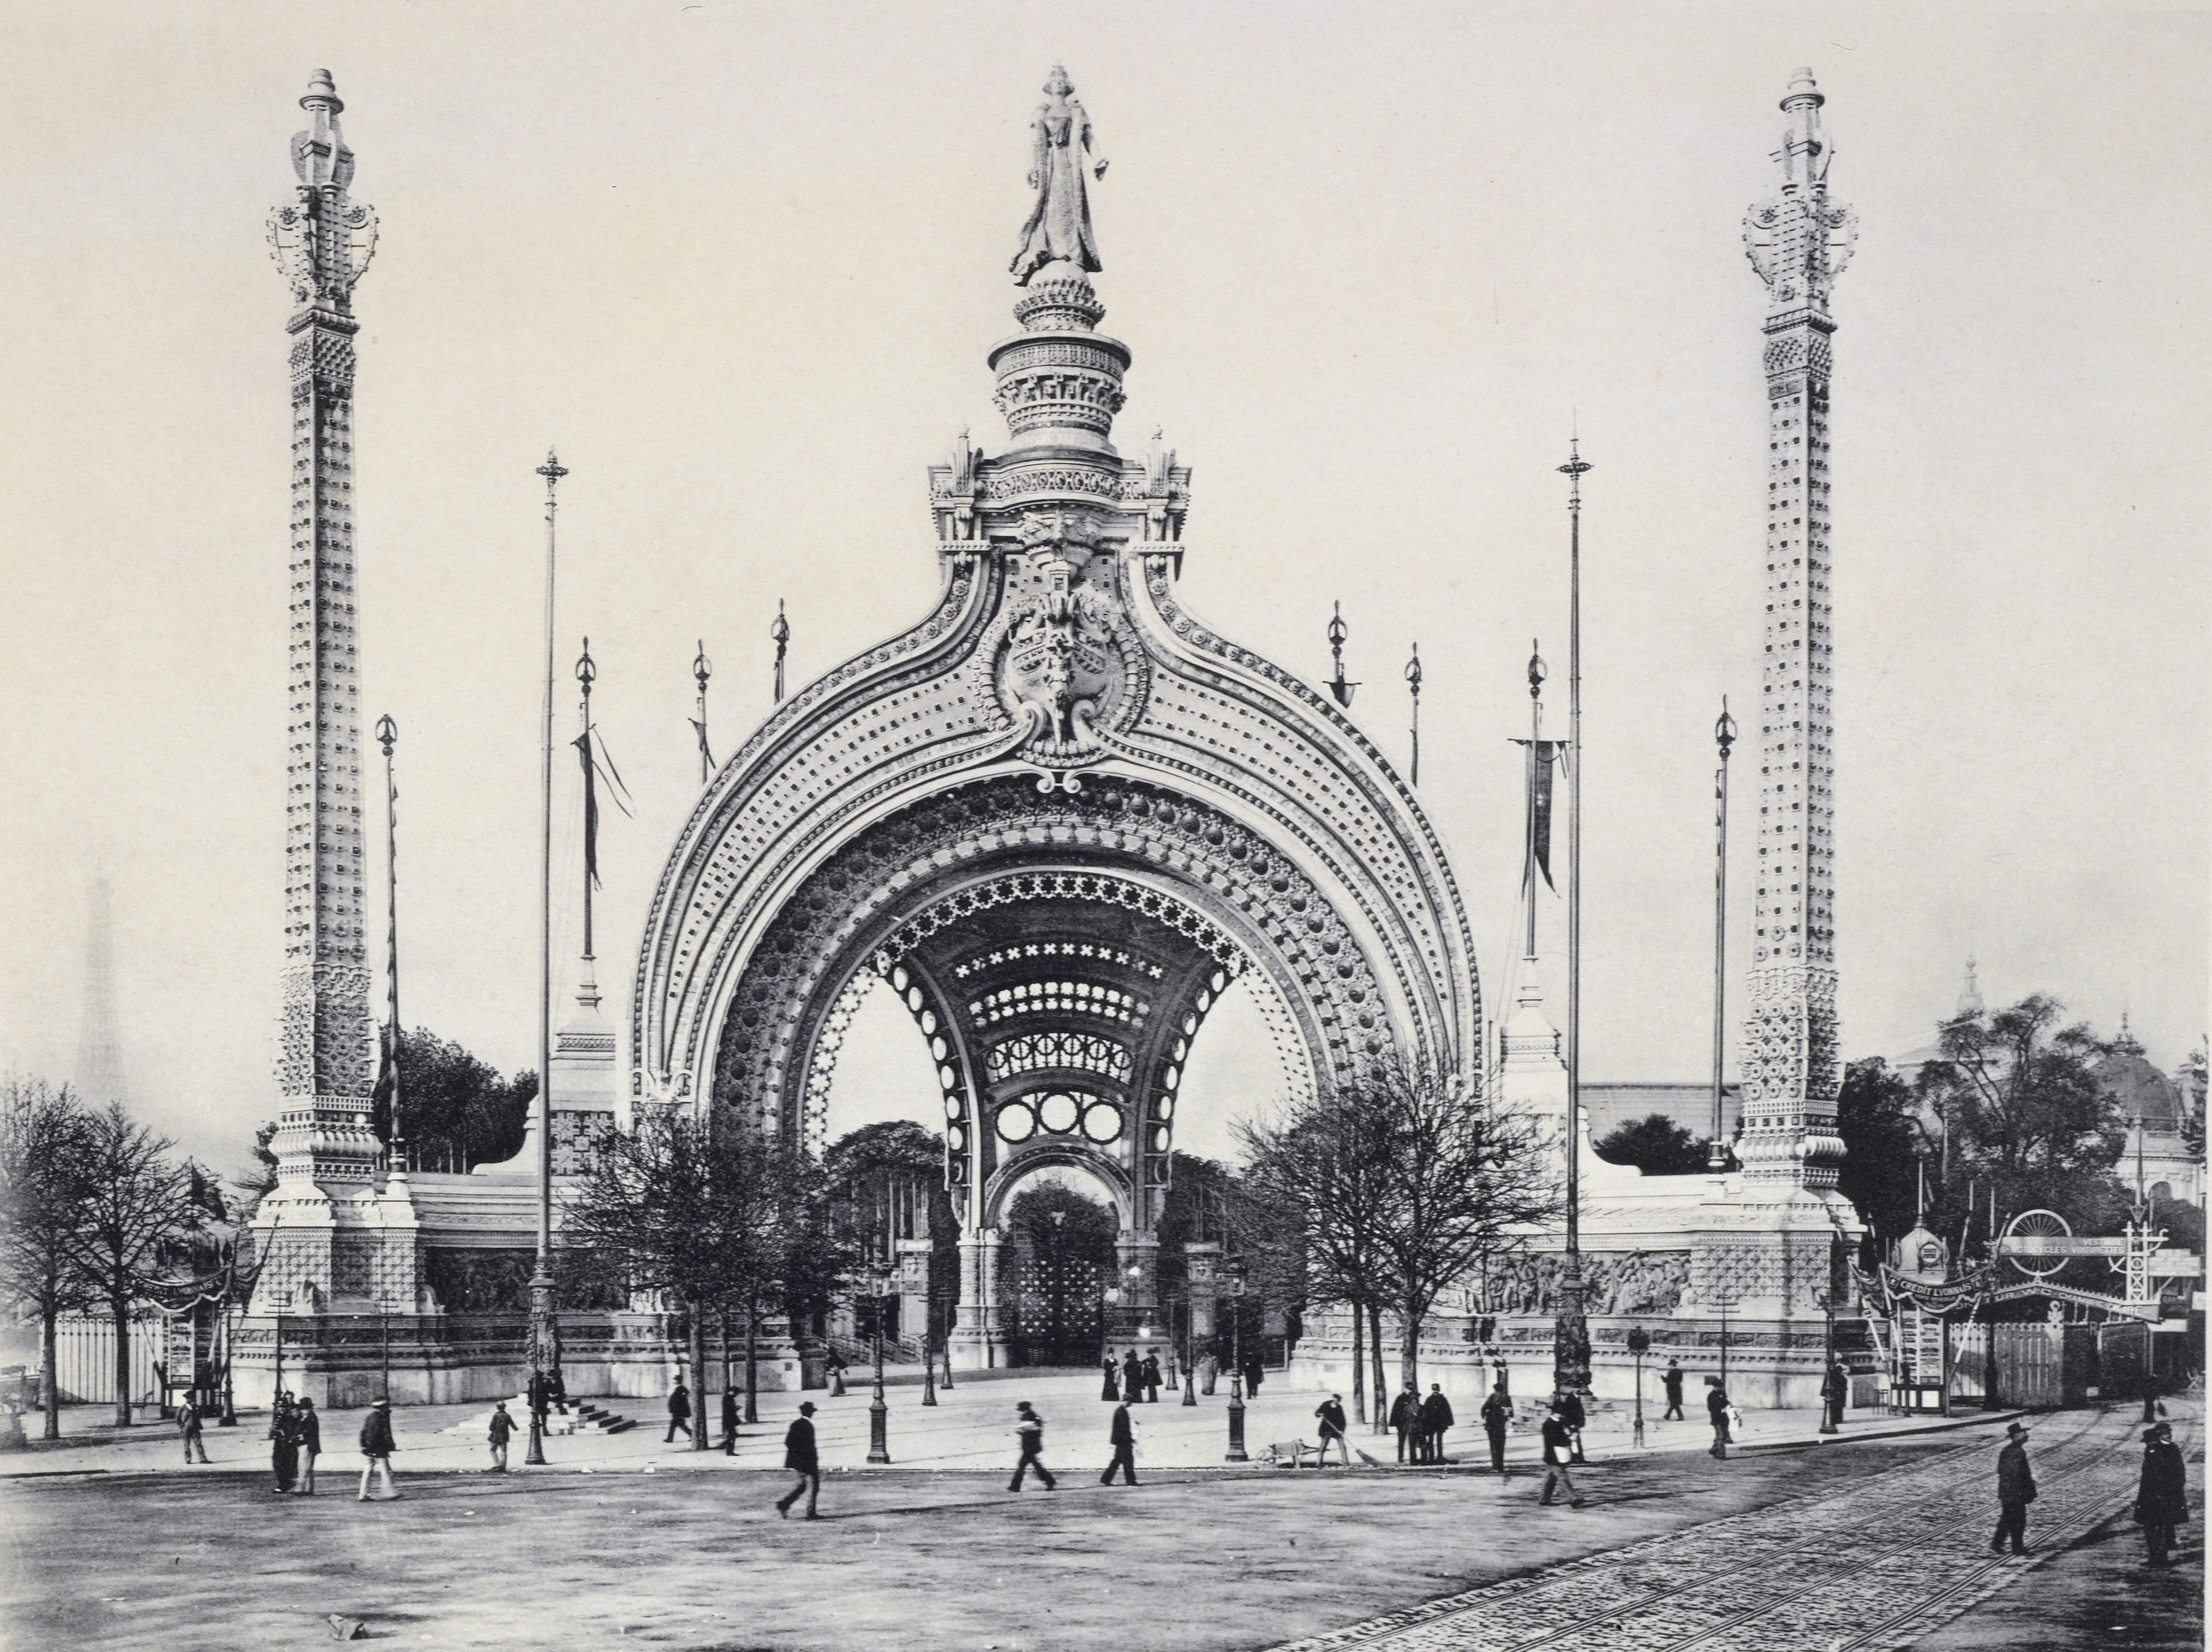
\includegraphics[height=4cm]{figures/porte_photograph.jpg} }}
    \subfloat{{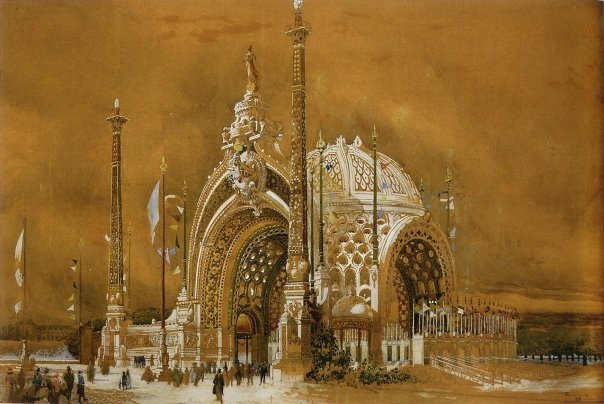
\includegraphics[height=4cm]{figures/porte_watercolor.jpg} }}
    \caption{Two renderings of the \textit{"Porte Binet"}, a monumental gate designed by Rene Binet for the 1900 Paris Exposition. Image sources: Photograph by Larger \cite{louis_porte_1900} and watercolor on paper by Binet \cite{binet_projet_1898}.}
    \label{fig:arch}
\end{figure}

\clearpage
\printbibliography

\end{document}
